\documentclass{article}
\usepackage[utf8]{inputenc}
\usepackage{listings}
\usepackage{multimedia} % to embed movies in the PDF file
\usepackage{graphicx}
\usepackage{comment}
\usepackage[english]{babel}
\usepackage{amsmath}
\usepackage{amsfonts}
\usepackage{wrapfig}
\usepackage{multirow}
\usepackage{verbatim}
\usepackage{float}
\usepackage{cancel}
\usepackage{caption}
\usepackage{subcaption}
\usepackage{/home/cade/Homework/latex-defs}
\usepackage{/home/cade/Homework/jlcode}


\title{AMATH 536 Problem Set 3}
\author{Cade Ballew \#2120804}
\date{May 6, 2022}

\begin{document}
	
\maketitle
	
\section{Problem 1}
Assume that there are $n_i$ resistance mutations providing resistance to drug $i$, and that the point mutation rate is $\mu$. We will further assume that there are no mutations that provide resistance to more than one of the drugs. Process is initiated at time 0 with a single cell sensitive to all drugs. All cells in the process have birth rate $b$ and death rate $d$, with $b>d$.

\subsection{Part a}
To calculate the expected number of cells resistant to all $n$ drugs at time $t$ arising through a single path $0 \to 1 \to 2 \to...\to n$, we first define 
\[
\alpha_j=\begin{cases}
(1-\mu n_{j+1})b-d, \quad &j=0,\ldots,n-1\\
b-d, \quad &j=n	
\end{cases}
\]
as the growth rate for type $j$ cells and
\[
\beta_j=\mu b n_j
\]
to be the mutation rate for type $j$ cells from type $j-1$ cells, $j=1,\ldots,n$. If $X_k(t)$ is the expected number of cells resistant to first $k$ drugs, then we have the system of ODEs
\begin{align*}
&X_0'(t)=\alpha_0X_0(t)\\
&X_j'(t)=\alpha_jX_j(t)+\beta_{j}X_{j-1}(t), \quad j=1,\ldots,n.
\end{align*}
For an initial condition, assume that we start with 1 cell with no mutations at time $t=0$, so $X_0(0)=1$ and $X_j(0)=0$ for $j=1,\ldots,n$. We tackle this system by means of the Laplace transform. Namely, we use the fact that 
\[
\mathcal{L}[f'(t)](s)=s\mathcal{L}[f](s)-f(0^+)
\]
and denote $\mathcal{L}[X_j(t)]=V_j(s)$ to find that our system becomes
\begin{align*}
	&sV_0(s)-1=\alpha_0V_0(s)\\
	&sV_j(s)=\alpha_jV_j(s)+\beta_{j}V_{j-1}(s), \quad j=1,\ldots,n
\end{align*}
which a recurrence relation that is easily solvable. Namely,
\begin{align*}
	&V_0(s)=\frac{1}{s-\alpha_0}\\
	&V_j(s)=\frac{\beta_{j}V_{j-1}(s)}{s-\alpha_j}, \quad j=1,\ldots,n
\end{align*}
which can be recursively found to have form
\[
V_j(s)=\frac{1}{s-\alpha_0}\prod_{k=1}^{j}\frac{\beta_k}{s-\alpha_k}
\]
for $j=1,\ldots,n$. If we adopt the convention that $\beta_0=1$, this can be written as
\[
V_j(s)=\prod_{k=0}^{j}\frac{\beta_k}{s-\alpha_k}
\] 
for all $j=0,\ldots,n$. To compute the inverse transform, we use the general partial fraction decomposition formula to write 
\begin{align*}
	\prod_{k=0}^{j}\frac{1}{s-\alpha_k}=\sum_{k=0}^{j}\frac{1}{Q'(\alpha_k)}\frac{1}{s-\alpha_k}
\end{align*}
where 
\[
Q(s)=\prod_{\ell=0}^{j}(s-\alpha_\ell),
\]
so
\[
Q'(s)=\sum_{k=0}^j\left(\prod_{\ell=0,\ell\neq k}^{j}(s-\alpha_\ell)\right)
\]
and
\[
Q'(\alpha_k)=\prod_{\ell=0,\ell\neq k}^{j}(\alpha_k-\alpha_\ell).
\]
Thus,
\begin{align*}
V_j(s)=\left(\prod_{k=0}^{j}\beta_k\right)\sum_{k=0}^{j}\frac{1}{(s-\alpha_k)\prod_{\ell=0,\ell\neq k}^{j}(\alpha_k-\alpha_\ell)}.
\end{align*}
Now, use that in general
\[
\mathcal{L}^{-1}\left[\frac{1}{s-d}\right]=e^{dt}
\]
for a constant $d$ and use the linearity of the Laplace transform to get that
\[
X_j(t)=\left(\prod_{k=0}^{j}\beta_k\right)\sum_{k=0}^{j}\frac{e^{\alpha_k t}}{\prod_{\ell=0,\ell\neq k}^{j}(\alpha_k-\alpha_\ell)}.
\]
Finally, we can plug back in our coefficients for $j=1,\ldots,n-1$ while noting that 
\[
\alpha_k-\alpha_\ell=(1-\mu n_{k+1})b-d-((1-\mu n_{\ell+1})b-d)=b\mu(n_{\ell+1}-n_{k+1}).
\] 
for $k,\ell=0,\ldots,n-1$. Then,
\begin{align*}
X_j(t)&=\left(\prod_{k=1}^{j}\mu bn_k\right)\sum_{k=0}^{j}\frac{e^{((1-\mu n_{k+1})b-d)t}}{\prod_{\ell=0,\ell\neq k}^{j}b\mu(n_{\ell+1}-n_{k+1})}\\&=
\left((\mu b)^j\prod_{k=1}^{j}n_k\right)\sum_{k=0}^{j}\frac{e^{((1-\mu n_{k+1})b-d)t}}{(\mu b)^j\prod_{\ell=0,\ell\neq k}^{j}(n_{\ell+1}-n_{k+1})}\\&=
\left(\prod_{k=1}^{j}n_k\right)\sum_{k=0}^{j}\frac{e^{((1-\mu n_{k+1})b-d) t}}{\prod_{\ell=0,\ell\neq k}^{j}(n_{\ell+1}-n_{k+1})}.
\end{align*}
When $j=0$, we instead have simply that
\[
X_0(t)=e^{((1-\mu n_{1})b-d)t}
\]
as expected. When $j=n$, it is perhaps easiest to simply adopt the convention that $n_{n+1}=0$ so that we may use our prior analysis to write
\[
X_n(t)=\left(\prod_{k=1}^{n}n_k\right)\sum_{k=0}^{n}\frac{e^{((1-\mu n_{k+1})b-d) t}}{\prod_{\ell=0,\ell\neq k}^{n}(n_{\ell+1}-n_{k+1})}
\]
as before. Note that this does have the implicit assumption that the $n_k$s are distinct.

\subsection{Part b}
To condition on the survival of the process, we note that the surivial probability is $1-\frac{d}{b}$, so we set
\[
N=\frac{e^{(b-d)t}}{1-\frac{d}{b}}=\frac{b}{b-d}e^{(b-d)t},
\]
so we plug in 
\[
t=\frac{\log\left(\frac{rN}{b}\right)}{r}
\]
if we set $r=b-d$ and multiply our entire expression by the survival probability. Then,
\begin{align*}
X_n(N)&=\frac{b}{r}\left(\prod_{k=1}^{n}n_k\right)\sum_{k=0}^{n}\frac{e^{((1-\mu n_{k+1})b-d) \frac{\log\left(\frac{rN}{b}\right)}{r}}}{\prod_{\ell=0,\ell\neq k}^{n}(n_{\ell+1}-n_{k+1})}\\&=
\frac{b}{r}\left(\prod_{k=1}^{n}n_k\right)\sum_{k=0}^{n}\frac{\left(\frac{rN}{b}\right)^{((1-\mu n_{k+1})b-d)/r}}{\prod_{\ell=0,\ell\neq k}^{n}(n_{\ell+1}-n_{k+1})}
\end{align*}
%for $j=1,\ldots,n$ and 
%\[
%X_0(N)=\frac{b}{r}\left(\frac{rN}{b}\right)^{((1-\mu n_{1})b-d)/r}
%\]
where we have maintained our convention that $n_{n+1}=0$.

\subsection{Part c}
Now, we start with our expression from part a so that we may Taylor expand
\begin{align*}
e^{((1-\mu n_{k+1})b-d) t}=e^{rt}\sum_{s=0}^\infty\frac{(-\mu n_{k+1}bt)^s}{s!},
\end{align*}
so
\begin{align*}
X_n(t)&=\frac{b}{r}\left(\prod_{k=1}^{n}n_k\right)\sum_{k=0}^{n}\frac{e^{rt}\sum_{s=0}^\infty\frac{(-\mu n_{k+1}bt)^s}{s!}}{\prod_{\ell=0,\ell\neq k}^{n}(n_{\ell+1}-n_{k+1})}\\&=
\frac{b}{r}e^{rt}\left(\prod_{k=1}^{n}n_k\right)\sum_{k=0}^{n}\sum_{s=0}^\infty\frac{(\mu bt)^s}{s!}\frac{(-n_{k+1})^s}{\prod_{\ell=0,\ell\neq k}^{n}(n_{\ell+1}-n_{k+1})}\\&=
\frac{b}{r}e^{rt}\left(\prod_{k=1}^{n}n_k\right)\sum_{s=0}^\infty\frac{(\mu bt)^s}{s!}\sum_{k=1}^{n+1}\frac{(-n_{k})^s}{\prod_{\ell=1,\ell\neq k}^{n+1}(n_{\ell}-n_{k})}\\&=
\frac{b}{r}e^{rt}\left(\prod_{k=1}^{n}n_k\right)\sum_{s=0}^\infty\frac{(\mu bt)^s}{s!}\sum_{k=1}^{n}\frac{(-n_{k})^{s}}{(-n_k)\prod_{\ell=1,\ell\neq k}^{n}(n_{\ell}-n_{k})}
\end{align*}
since we have the convention that $n_{n+1}=0$. Now, we can use the provided identity to find that 
\[
\sum_{k=1}^{n}\frac{(-n_{k})^{s}}{n_k\prod_{\ell=1,\ell\neq k}^{n}(n_{\ell}-n_{k})}=\begin{cases}
	\frac{1}{\prod_{\ell=1}^{n}n_\ell}, \quad &s=0\\
	0, \quad &1\leq s\leq n\\
	-1, \quad &s=n
\end{cases}
\]
which is nonzero only when $s=0,n$. We then truncate all terms where $s>n$ from our Taylor series which leaves us with
\begin{align*}
X_n(t)=\frac{b}{r}e^{rt}\left(\prod_{k=1}^{n}n_k\right)(-1)\left(\frac{1}{\prod_{\ell=1}^{n}n_\ell}+\frac{(\mu bt)^n}{n!}(-1)\right)=\frac{b}{r}e^{rt}\left(\left(\prod_{k=1}^{n}n_k\right)\frac{(\mu bt)^n}{n!}-1\right).
\end{align*}
Plugging back in $t=\frac{\log\left(\frac{rN}{b}\right)}{r}$,
\begin{align*}
X_n(N)&=\frac{b}{r}e^{\log\left(\frac{rN}{b}\right)}\left(\left(\prod_{k=1}^{n}n_k\right)\frac{(\mu b\frac{\log\left(\frac{rN}{b}\right)}{r})^n}{n!}-1\right)\\&=
N\left(\left(\prod_{k=1}^{n}n_k\right)\frac{(\mu b\log\left(\frac{rN}{b}\right))^n}{r^n n!}-1\right).
\end{align*}

\subsection{Part d}
To compute the expected number of cells resistant to all $n$ drugs, $1, 2, ...,n$ in a tumor containing $N$ cells, we note that there are $n!$ possible paths so we simply multiply our answer from part c by $n!$ to get
\[
N\left(\left(\prod_{k=1}^{n}n_k\right)\left(\frac{\mu b\log\left(\frac{rN}{b}\right)}{r}\right)^n-n!\right).
\]

\section{Problem 2}
\subsection{Part a}
We simulate the discrete-time branching process from the paper "Accumulation of driver and passenger mutations during tumor progression" with only type 1 and type 2 cells by taking the parameter values $u=3.4\times10^{-5}$, $T= 3$ days, and $s=0.4\%$ and letting $d_j=\half(1-s)^j$, $j=1,2$. We sample births, deaths, and mutations at each timestep via the multinomial distribution in (S2). The following are three simulations in which the process does not die out over 25 years. \\
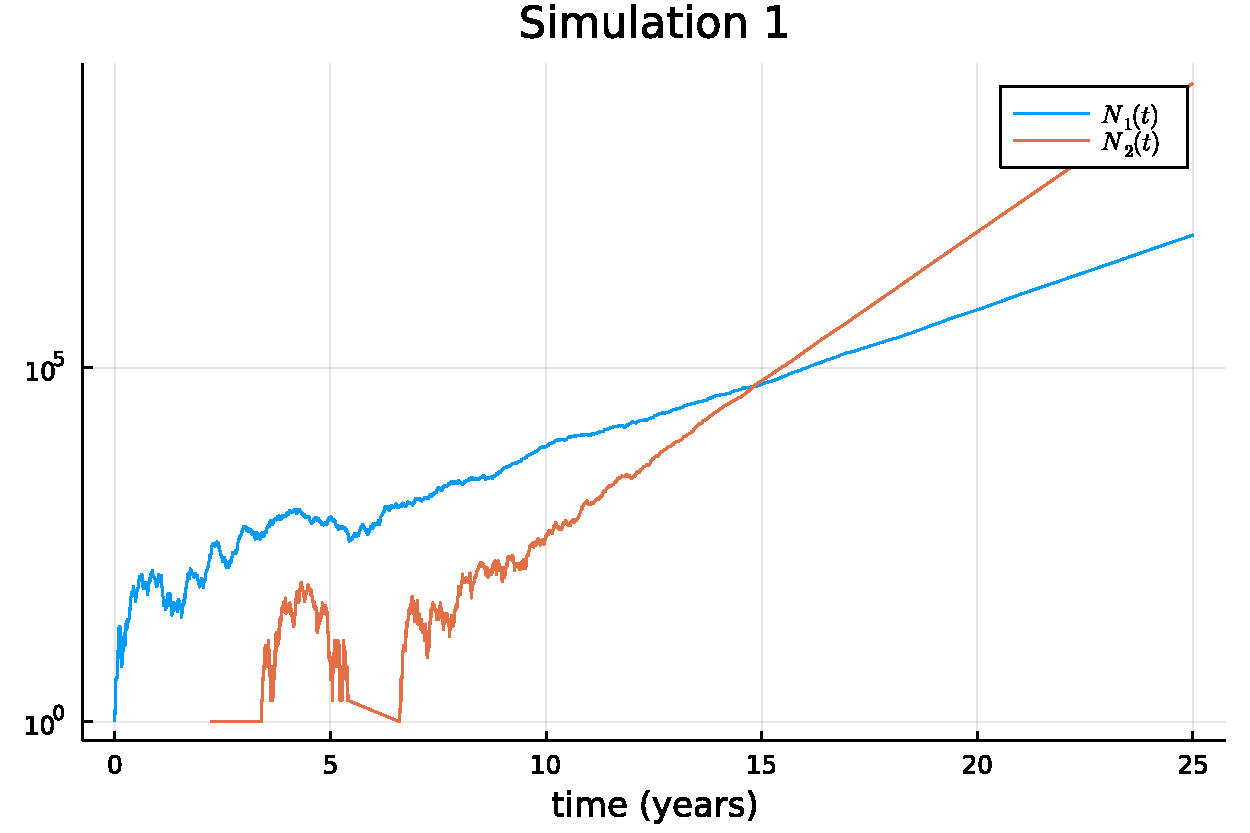
\includegraphics[scale=0.5]{sim1.pdf}\\
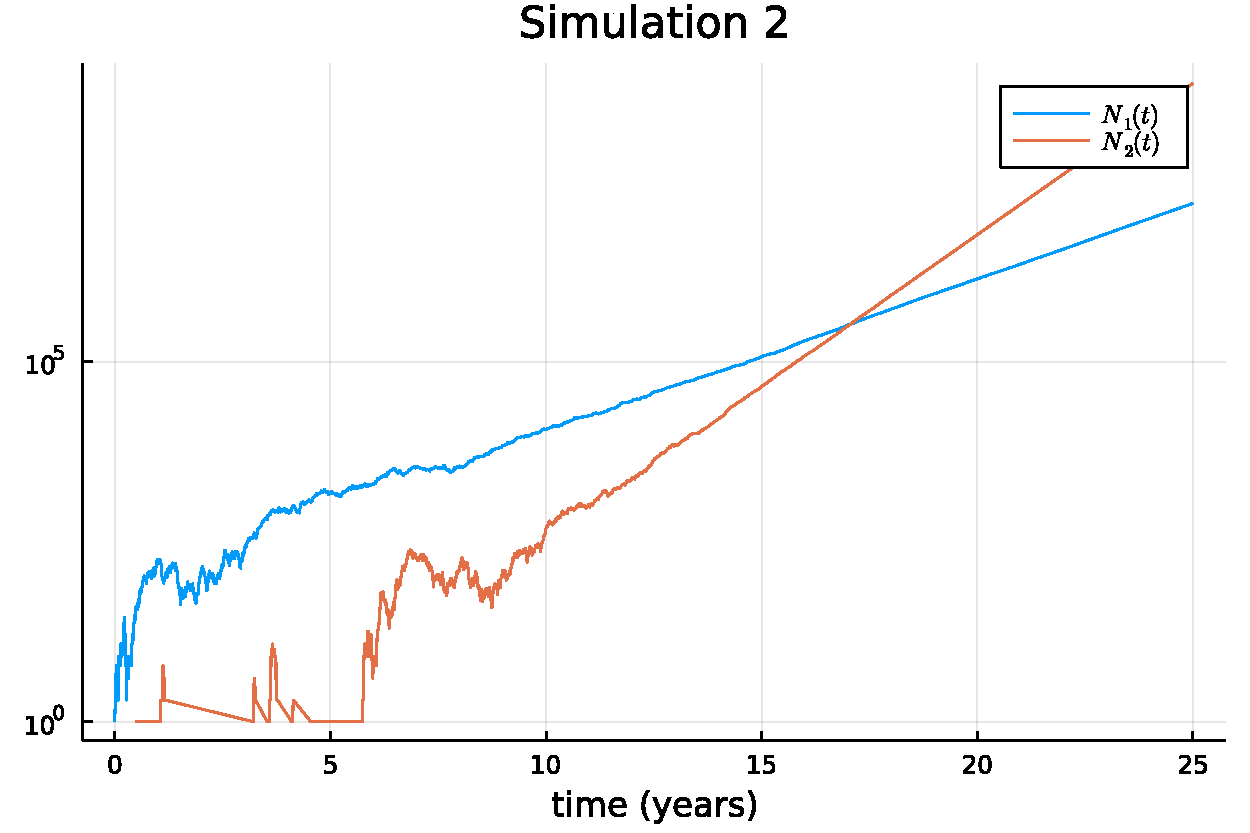
\includegraphics[scale=0.5]{sim2.pdf}\\
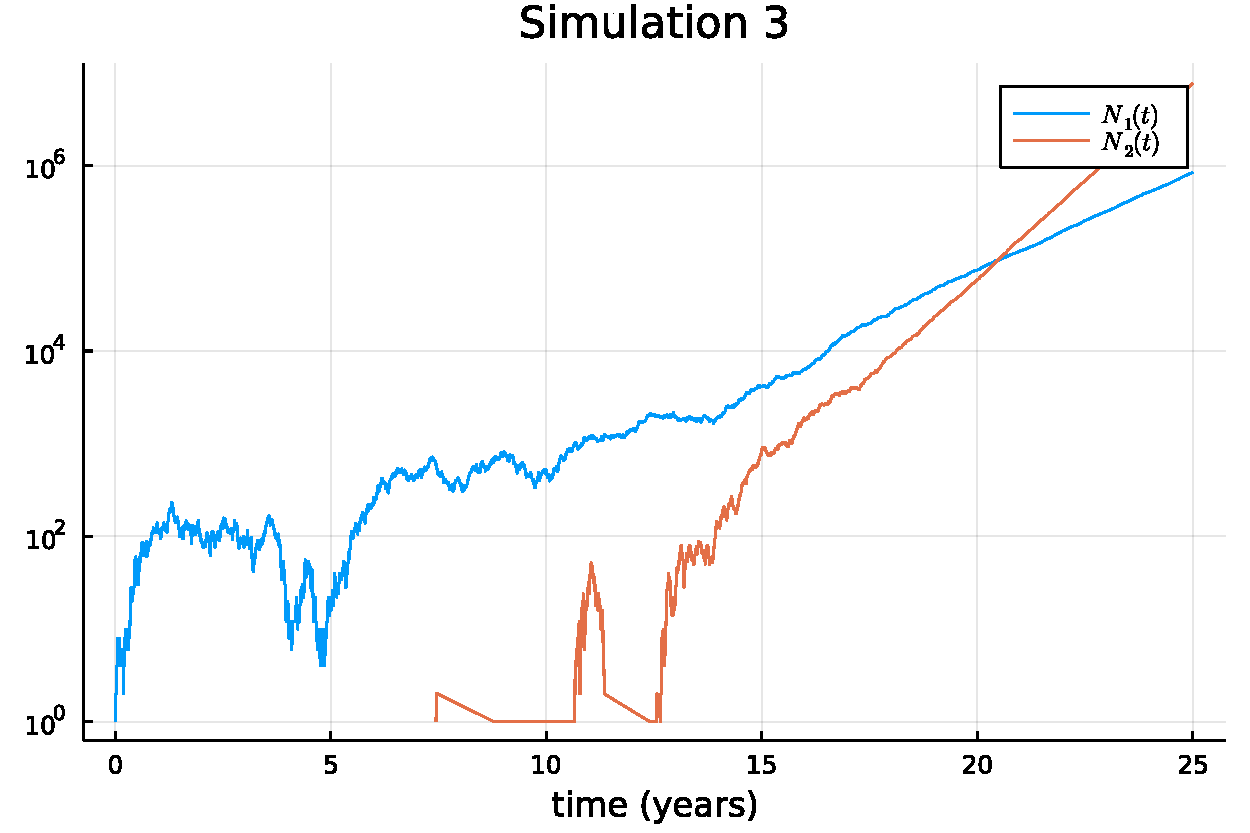
\includegraphics[scale=0.5]{sim3.pdf}

\subsection{Part b}
We now run the simulation 100000 times and produce the following plot of the average number of cells of each time present at each timestep.\\
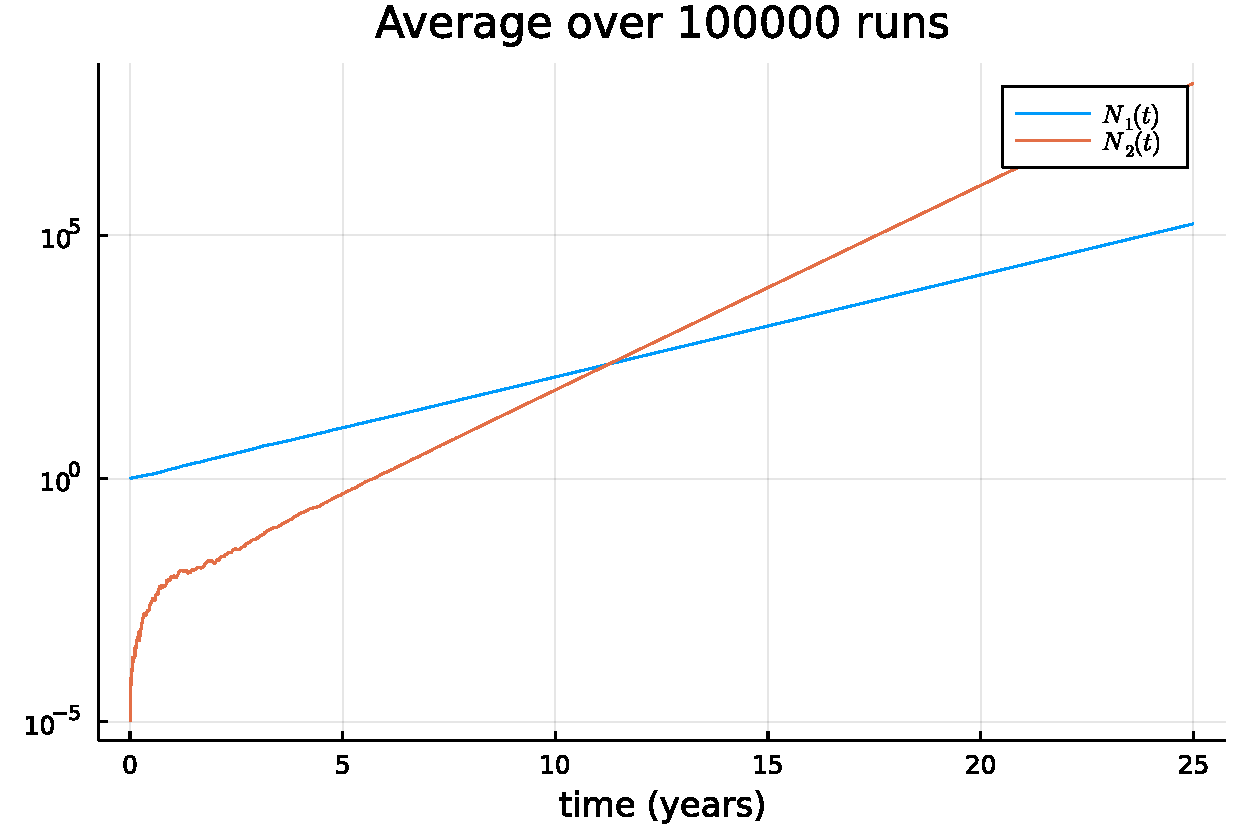
\includegraphics[scale=0.5]{avg.pdf}

\subsection{Part c}
To derive the average numbers of type 1 and type 2 cells in the process analytically, we keep with the notation of the paper by letting $u$ denote the mutation rate, $b_1,b_2$ the respective birth rates, and $d_1,d_2$ the respective death rates. If we let $x_t$ denote the expected number of type 1 cells at timestep $t$ (corresponding to time $tT$) and let $y_t$ denote the expected number of type 2 cells at timestep $t$, we have that 
\begin{align*}
x_t=x_{t-1}+b_1(1-u)x_{t-1}-d_1x_{t-1}\\
y_t=y_{t-1}+b_2y_{t-1}-d_2y_{t-1}+b_1ux_{t-1}.
\end{align*}
Note that we have assumed that type 2 cells are still able to mutate. Then, 
\[
x_t=(1+b_1(1-u)-d_1)x_{t-1},
\]
so we have that 
\[
x_t=(1+b_1(1-u)-d_1)^t
\]
since $x_0=1$. Then, we find that 
\begin{align*}
y_t=(1+b_2-d_2)y_{t-1}+b_1u(1+b_1(1-u)-d_1)^t.
\end{align*}
%Note that a general nonlinear recurrence $u^n=\alpha u^{n-1}+h_n$ has solution
%\begin{align*}
%	u^1&=\alpha u^0+h_1\\
%	u^2&=\alpha^2u^0+\alpha h_1+h_2\\
%	u^3&= \alpha^3u^0+\alpha^2 h_1+\alpha h_2+h_3\\
%	&\vdots\\
%	u^n&=\alpha^n u^0+\sum_{j=1}^{n}\alpha^{n-j}h_{j}.
%\end{align*}
%Since $y_0=0$, we have that
%\begin{align*}
%y_t&=\sum_{j=1}^{t}(1+b_2(1-u)-d_2)^{t-j}b_1u(1+b_1(1-u)-d_1)^j\\&=
%b_1u(1+b_2(1-u)-d_2)^t\sum_{j=1}^{t}\left(\frac{1+b_1(1-u)-d_1}{1+b_2(1-u)-d_2}\right)^j\\&=
%b_1u(1+b_2(1-u)-d_2)^t\frac{1+b_1(1-u)-d_1}{1+b_2(1-u)-d_2}\frac{1-\left(\frac{1+b_1(1-u)-d_1}{1+b_2(1-u)-d_2}\right)^t}{1-\left(\frac{1+b_1(1-u)-d_1}{1+b_2(1-u)-d_2}\right)}\\&=
%b_1u(1+b_2(1-u)-d_2)^{t-1}(1+b_1(1-u)-d_1)\cdot\\&\frac{(1+b_2(1-u)-d_2)^t-(1+b_1(1-u)-d_1)^t}{(1+b_2(1-u)-d_2)-(1+b_1(1-u)-d_1)}\frac{1+b_2(1-u)-d_2}{(1+b_2(1-u)-d_2)^{t}}\\&=
%b_1u(1+b_1(1-u)-d_1)\frac{(1+b_2(1-u)-d_2)^t-(1+b_1(1-u)-d_1)^t}{(b_2-b_1)(1-u)-(d_2-d_1)}
%\end{align*}
We can use Mathematica to solve this recurrence relationship (noting that $y_0=0$) which gives that
\[
y_t=\frac{b_1u((1+b_2-d_2)^t-(1+b_1(1-u)-d_1)^t)}{(b_2-d_2)-(b_1(1-u)-d_1)}.
\]
If we instead wish to have $t$ be the true time, we can simply write
\begin{align*}
&N_1(t)=(1+b_1(1-u)-d_1)^{t/T},\\
&N_2(t)=\frac{b_1u((1+b_2-d_2)^{t/T}-(1+b_1(1-u)-d_1)^{t/T})}{(b_2-d_2)-(b_1(1-u)-d_1)}.
\end{align*}
If we plot this, we observe the following\\
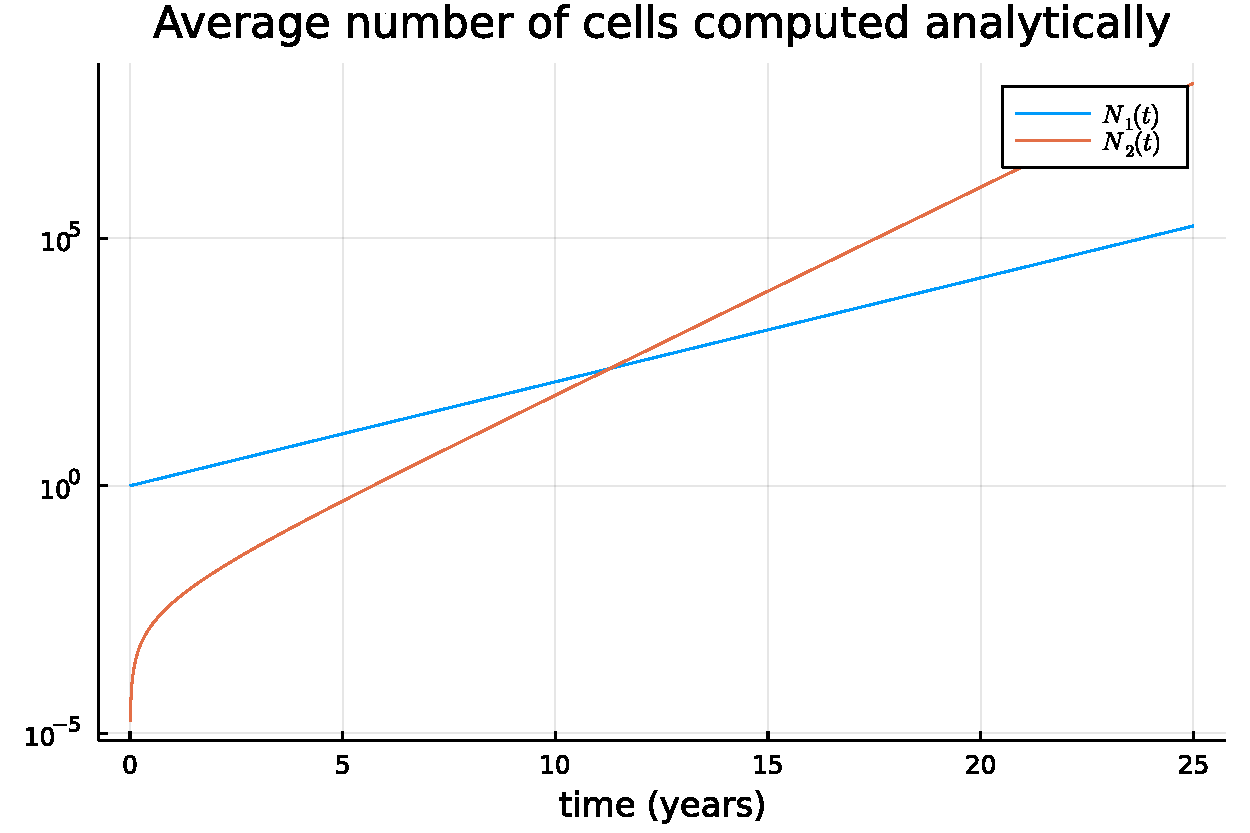
\includegraphics[scale=0.5]{true_avg.pdf}\\
In general, this seems to match what we observed in our 100000 trials. Using more trials would likely smooth out the curve for $N_2(t)$ to more closely match our analytical solution. 
%We see that the average of $N_1(t)$ seems to correspond well with what we observed numerically while the average of $N_2(t)$ seems to have a lower peak than what we observed. This is likely because $N_2(t)$ has a very high variance at later times, so despite having 100000 runs of our simulation, we still have not converged to the true average. 

\section{Appendix A}
The following Julia code is used for problem 2.
\jlinputlisting{Problem2.jl}
The following line of Mathematica code is used in problem 2 part c.
\begin{lstlisting}[language=Mathematica]
RSolve[{y[t + 1] == (1 + b - d) y[t] + au (1 + a (1 - u) - c), 
	y[0] == 0}, y[t], t]	
\end{lstlisting}
\end{document}
